\documentclass{article}

\usepackage{coursenotes}

\set{AuthorName}{TC Fraser}
\set{Email}{tcfraser@tcfraser.com}
\set{Website}{www.tcfraser.com}
\set{ClassName}{Topics in Condensed Matter}
\set{School}{University of Waterloo}
\set{CourseCode}{Phys 435}
\set{InstructorName}{Anton Burkov}
\set{Term}{Winter 2017}
\set{Version}{1.0}

\draftprofile[TC Fraser]{TC}{Red}

\begin{document}

\titlePage

\tableOfContents

\disclaimer

\section{Toy Model of a Solid}

\todo[TC]{Type up notes for first class}

\begin{center}
    \begin{tikzpicture}
        \foreach \i in {1,...,7}
        {
            \node[draw, fill, circle, inner sep=1pt] (\i) at (\i,0) {};
        }
        \draw[] (1) -- node[above]{$t$} (2);
        \draw[] (2) -- node[above]{$t$} (3);
        \draw[] (3) -- node[above]{$t$} (4);
        \draw[] (4) -- node[above]{$t$} (5);
        \draw[] (5) -- node[above]{$t$} (6);
        \draw[] (6) -- node[above]{$t$} (7);

        \draw[] (1) -- ++(-0.5, 0) node[left]{$\cdots$};
        \draw[] (7) -- ++(+0.5, 0) node[right]{$\cdots$};

        \draw[dashed] (3.5, -1) -- (3.5, 1);
        \draw[dashed] (4.5, -1) -- (4.5, 1);
        \draw[<->] (3.5, -0.7) -- node[below]{$a$} (4.5, -0.7);
    \end{tikzpicture}
\end{center}


Thus far we have been discussing a toy model of a solid in one dimension. By diagonalizing the Hamiltonian we were able to determine the energy levels of the various states,
\[ \varepsilon\br{k} = - 2 t \cos\br{ka} \eq \label{eq:single_energy__band}\]
Where $k$ is the wave-vector with $p = \hbar k$ as the ordinary linear momentum. Additionally, $t$ acts as a tunneling coefficient that dictates a tunneling \textit{rate} (up to a constant $\hbar$) for the electrons in the solid. Unlike free particles, the momentum $k$ in this toy model is confined to a discrete region.
\[ -\f{\pi}{a} \leq k < \f{\pi}{a} \]
This interval is called the \term{first Brillouin zone}.
To highlight this difference, we sometimes refer to $p$ in this model as the \term{crystal momentum}.\\

Moreover, the periodic boundary conditions used restrict $k$ to take on discrete and finite values,
\[ k = \f{2 \pi m}{Na} \qquad m = 0, \pm 1, \pm 2, \ldots \]
Where $L = Na$ is the size of the crystal, $N$ is the number of atoms and $a$ is the interval between two atoms in the solid.\\

The states that diagonalized the Hamiltonian are called \term{Bloch states} and are denoted $\ket{k}$ where,
\[ \ket{k} = \f{1}{\sqrt{N}} \sum_{n} \ket{n} e^{i k na} \]
Which is a \term{lattice Fourier transform}. Since $k$ is confined to a finite interval, the energy levels are confined to a finite interval,
\[ \varepsilon_{\min} = - 2t \qquad \varepsilon_{\max} = + 2t \]
The interval has a width of $\varepsilon_{\max} - \varepsilon_{\min} = 4t$ and is referred to as the allowed energy \textit{band}.

\begin{center}
\begin{tikzpicture}
    \pgfmathsetmacro{\axissize}{4};
    \pgfmathsetmacro{\plotsize}{3};
    \draw[->] (-\axissize,0) -- (+\axissize,0) node[right]{$k$};
    \draw[->] (0, -\axissize) -- (0,+\axissize) node[above]{$\vep\br{k}$};
    \draw[scale=1.0,domain=-pi:pi,smooth,variable=\k,red] plot ({\k/pi*\plotsize},{-2*cos(deg(\k))});
    \draw[dashed] (\plotsize, -\axissize) -- node[above right]{$\f{\pi}{a}$} (\plotsize,+\axissize);
    \draw[dashed] (-\plotsize, -\axissize) -- node[above left]{$-\f{\pi}{a}$} (-\plotsize,+\axissize);
    \draw[-] (-0.1,-2) -- (+0.1,-2) node[right]{$-2t$};
\end{tikzpicture}
\end{center}

How many states does the band contain. Given that $k$ is discrete and bounded,
\[ -\f{\pi}{a} \leq \f{2 \pi m}{Na} = k < \f{\pi}{a} \]
Implies,
\[ -\f{N}{2} \leq m < \f{N}{2} \]
Therefore there are $N$ distinct waves of $m$. The total number states per band is thus $2N$ where $N$ is the number of primitive unit cells in the crystal.\\

Suppose now that we have $1$ electron per atom (instead of $1$ electron in total). We recall the \term{Pauli principle} which states that only $1$ electron can occupy a given state in a band. Since there are $N$ electrons and $2N$ states, the band is \textit{half-filled}.
\begin{center}
\begin{tikzpicture}
    \pgfmathsetmacro{\axissize}{4};
    \pgfmathsetmacro{\plotsize}{3};
    \draw[->] (0,0) -- (+\axissize,0) node[right]{$T$};
    \draw[->] (0, 0) -- (0,+\axissize) node[above]{$\rho\br{T}$};
    \draw[scale=1.0,domain=0.25:\plotsize,smooth,variable=\T,red] plot ({\T},{1/\T});
\end{tikzpicture}
\end{center}

When the electrons occupy all of the lowest possible energy states, we fill all of the negative energy states and the positive energy states remain vacant. This separation defines the \term{Fermi energy} for this system where occurs at $\vep\tsb{F} = 0$. In order to find the state that corresponds to this upper limit one needs to solve,
\[ \vep\br{k} = \vep\tsb{F} = 0 \implies -2t \cos\br{ka} = 0 \]
Therefore the value of $k$ that solves this equation is,
\[  k = \pm \f{\pi}{2a} = \pm k\tsb{F}\]
Where $k\tsb{F}$ is given a special name: the \term{Fermi wave-vector} (Fermi momentum).
\begin{align*}
    \abs{k} < k\tsb{F} &: \text{filled states}\\
    \abs{k} > k\tsb{F} &: \text{empty states}
\end{align*}
The \term{Fermi surface} defines the surface in momentum space separating the filled states from the unfilled states. Most of the observed properties of metals follow from the existence of the Fermi surface. \\

This concept is so important that it is worth measuring the volume \text{in momentum space} corresponding to the filled states. This is the volume enclosed by the Fermi surface. In this example, the volume in momentum space is characterized by the $2 k\tsb{F}$ interval. Since $k = 2\pi m / Na$, the volume per single $k$-value is $2 \pi / Na$. Letting $n$ be the density of electrons, we can compute the total number of electrons:
\[ n N a = 2 \f{2k\tsb{F}}{2 \pi / Na} \]
Which allows one to calculate $k\tsb{F}$,
\[ k\tsb{F} =\f{\pi}{2} n \]
Which makes sense for this model because there is one electron per atom making $n = 1/a$.
This result is called \term{Luttinger's theorem} which states that the volume enclosed by the Fermi surface (sometimes called the Fermi sea) is directly proportional to the electron density. \\

This toy model actually describes a real solid called polyacetylene. Polyacetylene consists of weakly-interacting chains of CH units.
\begin{align*}
    \text{C} &: 1s^2 2s^2 2p^2 \qquad \text{4 valence electrons}\\
    \text{H} &: 1s^1
\end{align*}

Electrons found in the inner orbitals of the atoms are tightly bound to their nuclei and therefore only the valence electrons in carbon are free to travel throughout the lattice.

\begin{center}
    \includegraphics[width=\linewidth]{figures/polyacetylene.png}
\end{center}

Three of the valence electrons are engaged in bonding with neighboring carbon and hydrogen atoms while the $4$-th one is free to move around. As it turns out, the bonds between carbon atoms possess alternating tunneling amplitudes.

\begin{center}
    \begin{tikzpicture}
        \foreach \i in {1,...,7}
        {
            \node[draw, fill, circle, inner sep=1pt] (\i) at (\i,0) {};
        }
        \draw[]       (1) -- node[above]{$t_2$} (2);
        \draw[double] (2) -- node[above]{$t_1$} (3);
        \draw[]       (3) -- node[above]{$t_2$} (4);
        \draw[double] (4) -- node[above]{$t_1$} (5);
        \draw[]       (5) -- node[above]{$t_2$} (6);
        \draw[double] (6) -- node[above]{$t_1$} (7);


        \draw[double] (1) -- ++(-0.5, 0) node[left]{$\cdots$};
        \draw[]       (7) -- ++(+0.5, 0) node[right]{$\cdots$};

        \draw[dashed] (3.5, -1) -- (3.5, 1);
        \draw[dashed] (5.5, -1) -- (5.5, 1);
        \draw[<->] (3.5, -0.7) -- node[below]{$2a$} (5.5, -0.7);
    \end{tikzpicture}
\end{center}

In Polyacetylene, the tunneling amplitude between the carbon atoms joined by a double bound is slightly higher $t_1 > t_2$. This is referred to as \term{Peierls instability}. \\

Since this deviation is only slight, let $2\de t = t_1 - t_2$ such that,
\[ t_1 = t + \de t \qquad t_2 = t - \de t \eq \label{eq:t1t2}\]
Another important difference is that the primitive unit cell has size $2a$ (instead of $a$). This two atom basis can be arranged on a lattice with lattice constant $2a$. This is referred to as a \term{Bravais lattice}. Notationally, we can describe any crystal as,
\[ \text{crystal} = \br{\text{basis}, \text{Bravais lattice}} \]

To describe an electron in this lattice, we need two indices: one to describe the unit cell the electron is in and one to describe which atom ($1$ or $2$) the electron is located at. Therefore the Hamiltonian needs to characterize a number of possible transitions,
\begin{itemize}
    \item $\ket{n, 2} \bra{n, 1}, \ket{n, 1} \bra{n, 2}$ tunneling within a unit cell (forward, backward)
    \item $\ket{n-1, 2} \bra{n, 1}, \ket{n, 1} \bra{n-1, 2}$ tunneling between unit cells (forward, backward)
\end{itemize}

\[ H = \sum_{n} \bc{ - t_1 \ket{n, 2} \bra{n, 1} - t_2 \ket{n-1, 2} \bra{n, 1} - t_1 \ket{n, 1} \bra{n, 2} - t_2 \ket{n, 1} \bra{n-1, 2}} \]

Just as before, we need to write $\ket{n, \al}$ in the momentum basis,
\[ \ket{n, \al} = \sum_{k} \ket{k,\al} \braket{k, \al}{n, \al} \]
Where $\braket{k, \al}{n, \al}$ is written as,
\[ \braket{k, \al}{n, \al} = \f{1}{\sqrt{N}} e^{- 2 i k n a} \]
It is important to note that here $N$ does not represent the total number of atoms; $N$ is the total number of unit cells (equivalently the total number of distinct $\ket{n, \al}$ states for \textit{fixed} $\al$). Moreover the extra factor of $2$ in the exponential is due to the increases unit cell size. In momentum space, the Hamiltonian can be written,
\begin{align*}
\eq \label{eq:H_polyacetylene}
\begin{split}
H
&= - t_1 \f{1}{N} \sum_{n} \sum_{k ,k'} \ket{k, 2}\bra{k', 1} e^{-2ikna}e^{2ik'na} \\
&\quad  - t_2 \f{1}{N} \sum_{n} \sum_{k ,k'} \ket{k, 2}\bra{k', 1} e^{-2ik\br{n-1}a}e^{2ik'na} \\
&\quad  - t_1 \f{1}{N} \sum_{n} \sum_{k ,k'} \ket{k, 1}\bra{k', 2} e^{-2ikna}e^{2ik'na} \\
&\quad  - t_2 \f{1}{N} \sum_{n} \sum_{k ,k'} \ket{k, 1}\bra{k', 2} e^{-2ikna}e^{2ik'\br{n-1}a}
\end{split}
\end{align*}

One again we need to make use of the following identity,
\[ \f{1}{N} \sum_{n}e^{-2i \br{k - k'}na} = \de_{k, k'} \eq \label{eq:crystal_ident_polyacetylene}\]
Each term in \cref{eq:H_polyacetylene} contains terms of the form of \cref{eq:crystal_ident_polyacetylene} which simply $H$ greatly,
\begin{align*}
\eq\label{eq:H_diag_k}
\begin{split}
H
&= - t_1 \sum_{k}\bc{\ket{k ,2} \bra{k, 1} + \ket{k, 1}\bra{k,2}} \\
&\quad - t_2 \sum_{k}\bc{\ket{k ,2} \bra{k, 1}e^{2ika} + \ket{k, 1}\bra{k,2}e^{-2ika}}
\end{split}
\end{align*}
Already we can see that unlike the previous model, the Hamiltonian is not yet diagonalize. At this point, we have only \textit{partially} diagonalized the Hamiltonian with respect to the index of the unit cell. What remains is to diagonalize the Hamiltonian with respect to the index of the \textit{atom} within a single unit cell (i.e. $\al = 1,2$). In order to do this, notice that \cref{eq:H_diag_k} can be written as,
\[ H = \sum_{k} H\br{k} \]
Where $H\br{k}$ is a $k$ dependent Hamiltonian. We will focus on this Hamiltonian henceforth.
\begin{align*}
\begin{split}
H\br{k}
&= - t_1 \bc{\ket{k ,2} \bra{k, 1} + \ket{k, 1}\bra{k,2}} \\
&\quad - t_2 \bc{\ket{k ,2} \bra{k, 1}e^{2ika} + \ket{k, 1}\bra{k,2}e^{-2ika}}
\end{split}
\end{align*}
For convenience, we will drop reference to $k$ within the states,
\begin{align*}
\eq\label{eq:H_of_k}
\begin{split}
H\br{k}
&= - t_1 \bc{\ket{2} \bra{1} + \ket{1}\bra{2}} \\
&\quad - t_2 \bc{\ket{2} \bra{1}e^{2ika} + \ket{1}\bra{2}e^{-2ika}}
\end{split}
\end{align*}
\Cref{eq:H_of_k} has the Hamiltonian of a $2$ level system. Therefore we can model this system as a spin-$1/2$ system using the \term{Pauli matrices}. Recall,
\begin{align*}
\eq \label{eq:pauli_matrices}
\begin{split}
\si_x &= \begin{pmatrix} 0 & 1 \\ 1 & 0 \end{pmatrix} = \ket{\uparrow} \bra{\downarrow} + \ket{\downarrow} \bra{\uparrow} \\
\si_y &= \begin{pmatrix} 0 & -i \\ i & 0 \end{pmatrix} = -i\ket{\uparrow} \bra{\downarrow} - \ket{\downarrow} \bra{\uparrow} \\
\si_z &= \begin{pmatrix} 1 & 0 \\ 0 & -1 \end{pmatrix} = \ket{\uparrow} \bra{\uparrow} - \ket{\downarrow} \bra{\downarrow}
\end{split}
\end{align*}
Using the following correspondence (which we refer to as a pseudo-spin),
\[ \ket{1} = \ket{\uparrow} \qquad \ket{2} = \ket{\downarrow} \]
We have that,
\begin{align*}
H\br{k}
&= -\bs{\br{t + \de t} + \br{t - \de t} e^{- 2 i k a}} \ket{\uparrow}\bra{\downarrow}\\
&\quad - \bs{\br{t + \de t} + \br{t - \de t} e^{2 i k a}} \ket{\downarrow}\bra{\uparrow}
\end{align*}
We now elect to write $e^{\pm 2 i ka}$ in terms of sines and cosines and isolate the real and imaginary components,
\begin{align*}
H\br{k}
&= -\bs{\br{t + \de t} + \br{t - \de t} \cos\br{2 k a}} \ket{\uparrow}\bra{\downarrow}\\
&\quad + i\br{t - \de t} \sin\br{2 k a} \ket{\uparrow}\bra{\downarrow} + \text{h.c.}
\end{align*}
Where `h.c.' refers to the Hermitian conjugate the the preceding terms. At this stage, we define some notation,
\begin{align*}
\eq \label{eq:dk}
\begin{split}
d_x \br{k} &= - \br{t + \de t} - \br{t - \de t} \cos\br{2 ka} \\
d_y \br{k} &= - \br{t - \de t} \sin\br{2 ka} \\
d_z \br{k} &= 0
\end{split}
\end{align*}
Where $\ve d$ can be written,
\[ \ve d \br{k} = \br{d_x \br{k}, d_y \br{k}, d_z\br{k}} \]
Making use of \cref{eq:pauli_matrices}, we can see that,
\[ \ket{\uparrow}\bra{\downarrow} = \f{1}{2}\br{\si_x + i \si_y} \]
Which means that the Hamiltonian is,
\[ H\br{k} = \ve d\br{k} \cdot \ve \si \]
This system is \textit{equivalent} to a spin-1/2 particle in a magnetic field of the form $\ve d\br{k}$. The eigenstates of $H\br{k}$ correspond to $\ba{\ve \si}$ along $\ve d$ or in the opposite direction to $\ve d$,
\[ \vep_{\pm}\br{k} = \pm \abs{\ve d \br{k}} \]
This is contrasting to the previous model; before we had a \textit{single} energy band pursuant to \cref{eq:single_energy__band}, but here we have \textit{two energy bands}. This result can be generalized to the following observation:
\begin{center}
    \textit{Every atom in the unit cell will give rise to a separate band.}
\end{center}
Explicitly, $\abs{\ve d \br{k}}^2$ can be calculated from \cref{eq:dk},
\[ \abs{\ve d \br{k}}^2 = d_x^2 \br{k} + d_y^2 \br{k} + d_z^2 \br{k} = 4 t^2 \cos^2 \br{ka} + 4 \de t^2 \sin^2 \br{ka} \]
Which makes the two bands have the form,
\[ \vep_{\pm}\br{k} = \pm 2 \sqrt{t^2 \cos^2\br{ka} + \de t^2 \sin^2\br{ka}} \]
Which when plotted is,
\begin{center}
\begin{tikzpicture}
    \pgfmathsetmacro{\axissize}{4};
    \pgfmathsetmacro{\plotsize}{3};
    \pgfmathsetmacro{\dt}{0.65};
    \draw[->] (-\axissize,0) -- (+\axissize,0) node[right]{$k$};
    \draw[->] (0, -\axissize) -- (0,+\axissize) node[above]{$\vep\br{k}$};
    \draw[scale=1.0,domain=-pi/2:pi/2,smooth,variable=\k,red] plot ({2 *\k/pi*\plotsize},{-2*sqrt(cos(deg(\k))^2 + 0.1*sin(deg(\k))^2)});
    \draw[scale=1.0,domain=-pi/2:pi/2,smooth,variable=\k,red] plot ({2 *\k/pi*\plotsize},{2*sqrt(cos(deg(\k))^2 + 0.1*sin(deg(\k))^2)});
    \draw[dashed] (\plotsize, -\axissize) -- node[above right]{${\pi}/{2a}$} (\plotsize,+\axissize);
    \draw[dashed] (-\plotsize, -\axissize) -- node[above left]{$-{\pi}/{2a}$} (-\plotsize,+\axissize);
    \draw[] (-0.1,-2) -- (+0.1,-2) node[right]{$-2t$};
    \draw[] (-0.1,2) -- (+0.1,2) node[right]{$2t$};
    \draw[] (\plotsize-0.1, \dt) -- (\plotsize+0.1, \dt) node[right]{$2\de t$};
    \draw[] (\plotsize-0.1, -\dt) -- (\plotsize+0.1, -\dt) node[right]{$-2\de t$};
    \draw[] (-\plotsize-0.1, \dt) -- (-\plotsize+0.1, \dt) node[left]{$2\de t$};
    \draw[] (-\plotsize-0.1, -\dt) -- (-\plotsize+0.1, -\dt) node[left]{$-2\de t$};
    \draw[|<->|] (\plotsize-0.3, \dt) -- node[left]{$4 \de t$} (\plotsize-0.3, -\dt);
\end{tikzpicture}
\end{center}

Notice that the first Brillouin zone is $\f{\pi}{2a} \leq k \leq \f{\pi}{2a}$ is \textit{smaller} than it was previously. In this model, there is one electron per atom and thus two electrons per unit cell. Therefore there are $2N$ electrons. At zero temperature, the entire lower band is filled and the upper band is empty. This makes polyacetylene an \term{insulator} because it requires an energy of at least $4 \de t$ in order to transition an electron across the Fermi surface. \\

In the limit of the $\de t \to 0$ one should expect to recover \cref{eq:single_energy__band},
\[ \lim_{\de t \to 0}\vep_{\pm}\br{k} = \pm 2 \lim_{\de t \to 0}\sqrt{t^2 \cos^2\br{ka} + \de t^2 \sin^2\br{ka}} = \pm 2 t \cos\br{ka}  \]
As expected. Notice however the plot of $\ep\br{k}$ differs,
\begin{center}
\begin{tikzpicture}
    \pgfmathsetmacro{\axissize}{4};
    \pgfmathsetmacro{\plotsize}{3};
    \pgfmathsetmacro{\dt}{0};
    \draw[->] (-\axissize,0) -- (+\axissize,0) node[right]{$k$};
    \draw[->] (0, -\axissize) -- (0,+\axissize) node[above]{$\vep\br{k}$};
    \draw[scale=1.0,domain=-pi/2:pi/2,smooth,variable=\k,red] plot ({2 *\k/pi*\plotsize},{-2*sqrt(cos(deg(\k))^2)});
    \draw[scale=1.0,domain=-pi/2:pi/2,smooth,variable=\k,red] plot ({2 *\k/pi*\plotsize},{2*sqrt(cos(deg(\k))^2)});
    \draw[dashed] (\plotsize, -\axissize) -- node[above right]{${\pi}/{2a}$} (\plotsize,+\axissize);
    \draw[dashed] (-\plotsize, -\axissize) -- node[above left]{$-{\pi}/{2a}$} (-\plotsize,+\axissize);
    \draw[] (-0.1,-2) -- (+0.1,-2) node[right]{$-2t$};
    \draw[] (-0.1,2) -- (+0.1,2) node[right]{$2t$};
\end{tikzpicture}
\end{center}
The resolution between these two plots is to notice that in the polyacetylene model, the unit cell had with $2a$ instead of $a$. Therefore in momentum space, the plotted values for $k$ are bounded by $- \pi / 2a \leq k \leq \pi / 2a$ instead of $- \pi / a \leq k \leq \pi / a$. If one were to unravel the upper band into regions where $\abs{k} > \pi / 2a$ one would recover the initial model. \\

Heretofore, we have assumed that $\de t > 0$. If however we consider $\de t< 0$, then we transition from $t_1 > t_2$ to $t_2 > t_1$ pursuant to \cref{eq:t1t2}. And our diagram is adjusted

\begin{center}
    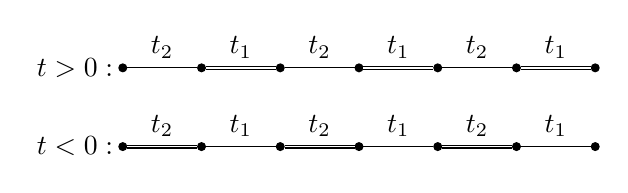
\begin{tikzpicture}
        \foreach \i in {1,...,7}
        {
            \node[draw, fill, circle, inner sep=1pt] (n\i) at (\i,0) {};
            \node[draw, fill, circle, inner sep=1pt] (p\i) at (\i,1) {};
        }
        \draw[]       (p1) -- node[above]{$t_2$} (p2);
        \draw[double] (p2) -- node[above]{$t_1$} (p3);
        \draw[]       (p3) -- node[above]{$t_2$} (p4);
        \draw[double] (p4) -- node[above]{$t_1$} (p5);
        \draw[]       (p5) -- node[above]{$t_2$} (p6);
        \draw[double] (p6) -- node[above]{$t_1$} (p7);
        \draw (p1) node[left]{$\de t > 0 : $};

        \draw[double] (n1) -- node[above]{$t_2$} (n2);
        \draw[]       (n2) -- node[above]{$t_1$} (n3);
        \draw[double] (n3) -- node[above]{$t_2$} (n4);
        \draw[]       (n4) -- node[above]{$t_1$} (n5);
        \draw[double] (n5) -- node[above]{$t_2$} (n6);
        \draw[]       (n6) -- node[above]{$t_1$} (n7);
        \draw (n1) node[left]{$\de t < 0 : $};
    \end{tikzpicture}
\end{center}

Therefore, the ground state of polyacetylene is doubly degenerate, corresponding to the two signs of $\de t$. As it turns out, this difference in sign is related to topological properties in momentum space. Upon examination of \cref{eq:dk} once can notice $\ve d$'s dependence on $\de t$. How does $\ve d\br{k}$ change as $k$ goes from $- \pi / 2a$ to $\pi  2a$?
\begin{align*}
\begin{split}
d_x \br{k} &= - \br{t + \de t} - \br{t - \de t} \cos\br{2 ka} \\
d_y \br{k} &= - \br{t - \de t} \sin\br{2 ka}
\end{split}
\end{align*}
Checking specific points,
\begin{align*}
d_x \br{\pm\f{\pi}{2a}} &= - \br{t + \de t} + \br{t - \de t} = - 2 \de t\\
d_y \br{\pm\f{\pi}{2a}} &= 0 \\
d_x \br{0} &= - \br{t + \de t} - \br{t - \de t} = 2 t\\
d_y \br{0} &= 0
\end{align*}
Plotted the case of $\de t >0$ in $d_y, d_x$ space,
\begin{center}
\begin{tikzpicture}
    \pgfmathsetmacro{\axissize}{3};
    \pgfmathsetmacro{\t}{1};
    \pgfmathsetmacro{\dt}{0.1};
    \pgfmathsetmacro{\tick}{0.1};
    \draw[->] (-\axissize,0) -- (+\axissize,0) node[right]{$d_x$};
    \draw[->] (0, -\axissize) -- (0,+\axissize) node[above]{$d_y$};
    \draw[scale=1.0,domain=-pi/2:pi/2,smooth,variable=\k,red] plot ({- (\t + \dt) - (\t - \dt)*cos(deg(2*\k))},{- (\t - \dt)*sin(deg(2*\k))});
    \draw[] (-2*\t, -\tick) -- (-2*\t, \tick) node[above left]{$-2t$};
    \draw[] (-2*\dt, -\tick) -- (-2*\dt, \tick) node[above left]{$-2\de t$};
    \draw[] (- 2, 2) node[]{$\de t > 0$};
\end{tikzpicture}
\end{center}
It can be seen that when $\de t > 0$, the curve in $d_x, d_y$ does not enclose the origin $\ve d = 0$. Recalling that $\vep_{\pm}\br{k} = \pm \abs{\ve d \br{k}}$, as long as $\ve d\br{k} \neq 0$, there exists a energy gap between the two bands $\vep_{+}$ and $\vep_{-}$. Therefore for $\de t > 0$ polyacetylene is an ordinary insulator. However, in the case where $\de t < 0$,
\begin{center}
\begin{tikzpicture}
    \pgfmathsetmacro{\axissize}{3};
    \pgfmathsetmacro{\t}{1};
    \pgfmathsetmacro{\dt}{-0.1};
    \pgfmathsetmacro{\tick}{0.1};
    \draw[->] (-\axissize,0) -- (+\axissize,0) node[right]{$d_x$};
    \draw[->] (0, -\axissize) -- (0,+\axissize) node[above]{$d_y$};
    \draw[scale=1.0,domain=-pi/2:pi/2,smooth,variable=\k,red] plot ({- (\t + \dt) - (\t - \dt)*cos(deg(2*\k))},{- (\t - \dt)*sin(deg(2*\k))});
    \draw[] (-2*\t, -\tick) -- (-2*\t, \tick) node[above left]{$-2t$};
    \draw[] (-2*\dt, -\tick) -- (-2*\dt, \tick) node[above left]{$-2\de t$};
    \draw[] (- 2, 2) node[]{$\de t > 0$};
\end{tikzpicture}
\end{center}
It can be seen that the origin $\abs{\ve d} = 0$ is enclosed. This \textit{topological} difference is what leads us to call the $\de t < 0$ a \term{topological insulator} as apposed to an \term{ordinary insulator}.\\

Effectively, there is no possible way to continuously deform the Hamiltonian (i.e. changing $\de t$) without merging the two energy bands. \\

An observable feature of topological insulators becomes evident for the edge states at zero energy (i.e. in the middle of a band gap). In this case of polyacetylene, these states that are closest to the band gap are those that live on the edge of the Brillouin zone where $\abs{k - \pi / 2a}$ is small. In order to explore the physics of these regions, define $\de k$ such that,
\[ k = \f{\pi}{2a} + \de k \]
Where $\de k$ is small. In this case, the Hamiltonian $H\br{k} = \ve d \br{k} \cdot \ve \si$ can be expanded out explicitly,
\begin{align*}
    d_x\br{k}
    &= d_x\br{\f{\pi}{2a} + \de k} \\
    &= - \br{t + \de t} - \br{t - \de t} \cos \br{\pi + 2 \de k a} \\
    &= - \br{t + \de t} + \br{t - \de t} \cos \br{2 \de k a} \\
    &= - \br{t + \de t} + \br{t - \de t} + \s O \br{\br{\de k}^2} \\
    &\simeq - 2 \de t
\end{align*}
Similarly for $d_y$,
\begin{align*}
    d_y\br{k}
    &= d_y\br{\f{\pi}{2a} + \de k} \\
    &= - \br{t - \de t} \sin \br{\pi + 2 \de k a} \\
    &= \br{t - \de t} \sin \br{2 \de k a} \\
    &= \br{t - \de t} 2 \de k a + \s O \br{\br{\de k}^3} \\
    &\simeq 2 t \de k a
\end{align*}
Therefore,
\[ H\br{\de k} = - 2 \de t \si_x + 2 t a \de k \si_y \]
In order to draw familiarity with systems that have been studied previously, let use rename a number of terms,
\[ 2 \de t = m \qquad 2 t a = \hbar v_F\]
Where $m$ has units of energy and $v_F$ has units of velocity. The Hamiltonian can now be written as,
\[ H = - m \si_x + \hbar v_F \de k \si_y \]
Since $\hbar \de k$ has units of momentum, we simply label it $p$. Then the Hamiltonian can be written as,
\[ H = v_F p \si_y - m \si_x \]
Which is identical to the Dirac equation (1D) for a \textit{relativistic} particle of \textit{mass} $m$ and velocity $v_F$ in place of the speed of light $c$. These velocity $v_F$ is called the \term{Fermi velocity}.

\[ \vep_{\pm}\br{p} = \pm \sqrt{v_F^2 p^2 + m^2} \]

Consider the interface between $2$ polyacetylene samples $\de t > 0$ and $\de t < 0$. In the position basis $p \to - i \hbar \di_x$ we can write our Dirac Hamiltonian as,
\[ H = - i \hbar v_F \si_y \di_x - m\br{x} \si_x \]
Where $m$ has an $x$ dependence.

\[  H \psi = E \psi \]
With $E = 0$ localized near $x = 0$.
\[ \bs{- i \hbar v_F \si_y \di_x - m\br{x} \si_x} \psi\br{x} = 0 \]
Therefore we should look for a solution of the form,
\[ \psi\br{x} = e^{f\br{x}} \si_y \ket{z} \]
Where $\ket{z}$ is written in $\si_z$ basis,
\[ \ket{z} = z_{\uparrow} \ket{\uparrow} + z_{\downarrow} \ket{\downarrow} \]
\[ \si_{z}\ket{\uparrow} = + \ket{\uparrow} \qquad \si_{z}\ket{\downarrow} = - \ket{\downarrow} \]
Using $\si_y^2 = \ident$ and $\si_x \si_y = i \si_z$,
\[ \bs{i \hbar v_F \si_y \der{f}{x} + i m\br{x} \si_z} e^{f\br{x}}\ket{z} = 0 \]
Dropping the exponential $e^{f\br{x}}$,
\[ \bs{i \hbar v_F \si_y \der{f}{x} + i m\br{x} \si_z} \ket{z} = 0 \]
Adjusting the constant coefficients,
\[ \bs{\der{f}{x} + \f{m\br{x}}{\hbar v_F} \si_z} \ket{z} = 0 \]
Therefore,
\[ \der{f}{x} = - \f{m\br{x}}{\hbar v_F} \]
Can be solved using,
\[ f\br{x} = - \f{1}{\hbar v_F} \intl_{0}^{x} \dif x' m\br{x'} \]
Where $m\br{0} = 0$. Altogether, the solution $\psi{x}$ can be written,
\[ \psi\br{x} = e^{- \f{1}{\hbar v_F} \int_{0}^{x} \dif x' m\br{x'}} \si_y \ket{\uparrow} \]
Since $\si_y \ket{\uparrow} = i \ket{\downarrow}$,
\[ \psi\br{x} = ie^{- \f{1}{\hbar v_F} \int_{0}^{x} \dif x' m\br{x'}}\ket{\downarrow} \]

\begin{center}
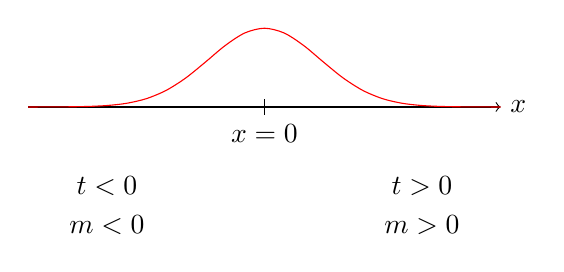
\begin{tikzpicture}
    \draw[->] (-3, 0) -- (3, 0) node[right]{$x$};
    \draw (0, -0.1) node[below]{$x = 0$} -- (0, 0.1);
    \draw (-2, -1) node[]{$\de t < 0$};
    \draw (-2, -1.5) node[]{$m < 0$};
    \draw (2, -1) node[]{$\de t > 0$};
    \draw (2, -1.5) node[]{$m > 0$};
    \draw[scale=1.0,domain=-3:3,smooth,variable=\x,red] plot ({\x},{exp(-\x*\x)});
\end{tikzpicture}
\end{center}

\section{Higher Dimensions}

A crystal is an infinite, periodic array of identical groups of atoms,
\[ \text{crystal} = \br{\text{basis}, \text{Bravais lattice}} \]

\begin{center}
    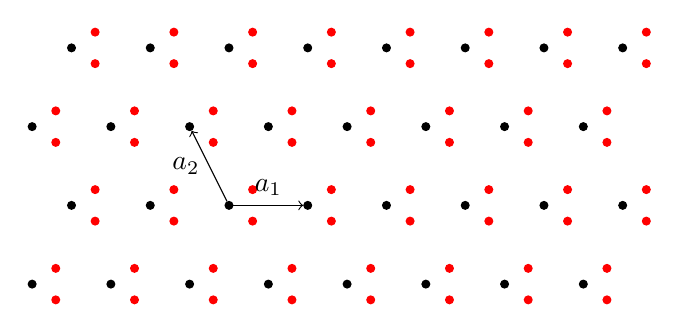
\begin{tikzpicture}
        \foreach \i in {1,...,8}
        {
            \foreach \j in {1,...,4}
            {
                \node[draw, fill, circle, inner sep=1pt] (\i\j) at ({\i+0.5*iseven(\j)},\j) {};
                \node[draw, fill, red, circle, inner sep=1pt] (a\i\j) at ({\i+0.5*iseven(\j)+0.3},\j-0.2) {};
                \node[draw, fill, red, circle, inner sep=1pt] (b\i\j) at ({\i+0.5*iseven(\j)+0.3},\j+0.2) {};
            }
        }
        \draw[->] (32) -- node[left]{$\ve a_2$} (33);
        \draw[->] (32) -- node[above]{$\ve a_1$} (42);
    \end{tikzpicture}
\end{center}

A \term{Bravais lattice} is all points in $\R^{3}$ ($\R^{2}, \R^{1}, \R^{n}$) such that,
\[ \ve R = n_1 \ve a_1 + n_2 \ve a_2 + n_3 \ve a_3 \]
Where $\ve a_1, \ve a_2, \ve a_3$ are the primitive translation vectors of the Bravais lattice. Moreover the coefficients $n_1, n_2, n_3$ are integers,
\[ n_1, n_2, n_3 = 0, \pm 1, \pm 2, \pm 3, \ldots \]
Typically, the choice for $\ve a_i$ is not unique. However, the best choice for the primitive transition vectors is typically the one that exhibits the most symmetry. \\

The \term{primitive unit cell} is the parallelepiped defined by the primitive translation vectors.\\

A Special type of unit cell, usually the most convenient, is the \term{Wigner-Seitz unit cell}. A WS unit cell is the region of space about a BL point that are closer to this point than to any other BL point.


\end{document}